\documentclass[useAMS,usenatbib,referee,12pt]{article}
\usepackage[margin=1.0in]{geometry}
\usepackage{amsmath}
\usepackage{amssymb}
\usepackage{amsfonts}
\usepackage{parskip}
\usepackage[round]{natbib}
\usepackage{caption}
\usepackage{tabularx, booktabs}
\usepackage{float}
\usepackage{adjustbox}
\usepackage{multirow}
\usepackage{setspace}
\usepackage{listings}
\usepackage{verbatim}
\usepackage{appendix}

\newcommand{\pdet}{p^{(det)}}
\renewcommand{\thesection}{S-\arabic{section}}   % Label section with 'S-#'
\renewcommand{\thetable}{S-\arabic{table}}
\renewcommand{\thefigure}{S-\arabic{figure}}

\begin{document}

\section{Tables and Figures}

\begin{figure}[h!]\centering
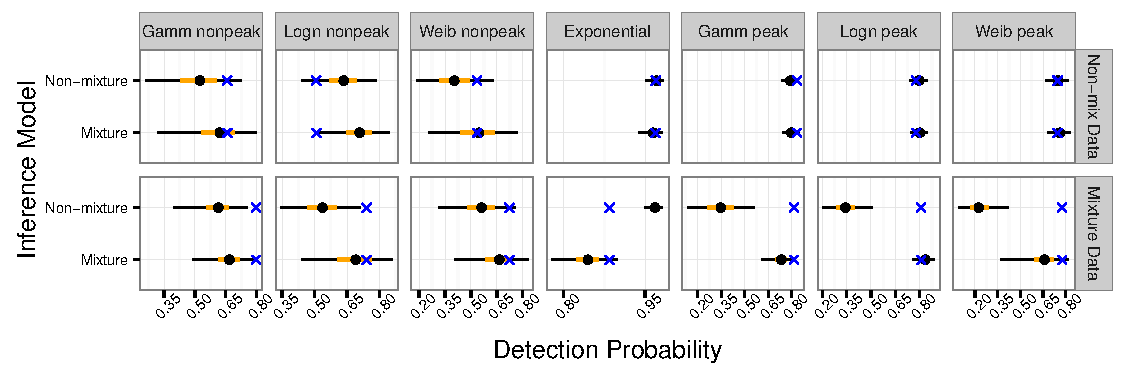
\includegraphics[width=0.98\textwidth]{Sims/SimFull/pdet_cater_correct.pdf}
\caption{\label{pdet_cater_correct} Sim3 caterpillar plots of posterior 50\% and 95\% credible intervals for the marginal probability of detection $\pdet$.  
Inference models come from the same family as the dataset but may differ in the presence/absence of a mixture component.  
Each column presents one family of simulated dataset.  
Upper plots show non-mixture datasets; lower plots show mixture datasets.  
`X' marks the expected marginal probability of detection based on true parameter values.}
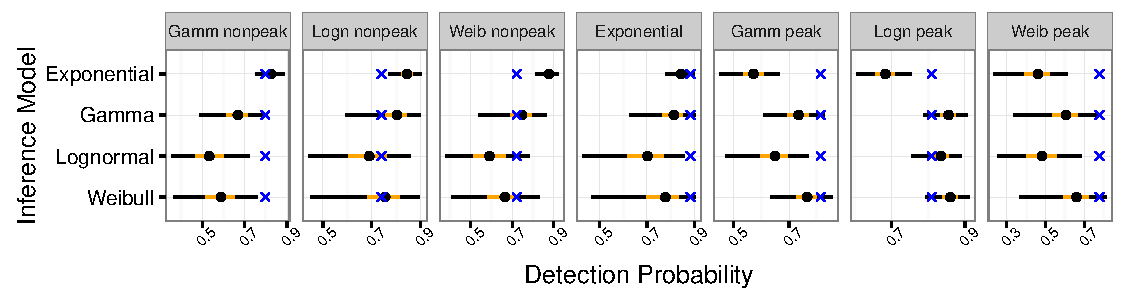
\includegraphics[width=0.98\textwidth]{Sims/SimFull/pdet_cater_family.pdf}
\caption{\label{pdet_cater_family}  Sim3 caterpillar plots of posterior 50\% and 95\% credible intervals for the marginal probability of detection $\pdet$. All data and inference models include mixtures.  
Each plot presents one simulated dataset.  
`X' marks the expected marginal probability of detection based on true parameter values.}
\end{figure}

\begin{table}[!ht]
\centering
\begin{tabular}{lll|ccc}
  \hline
Family & Mixture & Peaked & $\gamma$ & $\varphi$ & $\alpha$ \\ 
  \hline
Exponential & Non-mixture & &  & -1.827 &  \\ 
  & Mixture & & 0.65 & -2.138 &  \\ 
  \hline
  Gamma & Non-mixture & Non-peaked &  & -3.279 & 0.257 \\ 
  & & Peaked &  & -0.746 & 3.371 \\ 
  & Mixture & Non-peaked & 0.65 & -2.773 & 0.577 \\ 
  & & Peaked & 0.65 & -1.210 & 2.491 \\ 
  \hline
  Lognormal & Non-mixture & Non-peaked &  & -0.341 & 2.330 \\ 
  & & Peaked &  & -1.872 & 0.512 \\ 
  & Mixture & Non-peaked & 0.65 & -1.462 & 1.674 \\ 
  & & Peaked & 0.65 & -1.992 & 0.618 \\ 
  \hline
  Weibull & Non-mixture & Non-peaked &  & -1.165 & 0.418 \\ 
  & & Peaked &  & -2.042 & 1.829 \\ 
  & Mixture & Non-peaked & 0.65 & -2.063 & 0.687 \\ 
  & & Peaked & 0.65 & -2.201 & 1.621 \\ 
   \hline
\end{tabular}
\caption{\label{simvals}Table of parameter values used to generate data for: (i) the mixture vs. non-mixture simulation, and (ii) the constant vs. non-constant rate simulation.  Here $\gamma$ is a mixing parameter for the proportion of `hard to detect' individuals, $\varphi$ is the detection rate parameter, and $\alpha$ is the shape parameter.}
\end{table}

\begin{table}[ht]
\centering
\begin{tabular}{lllrrrrrrrrrrrrrrrr}
  \hline
Family & Mixture & Peak & Intercept$^A$ & $\beta^A_1$ & $\beta^A_2$ & $\beta^A_3$ & $\beta^A_4$ & Intercept$^D$ & $\beta^D_1$ & $\beta^D_2$ & $\beta^D_3$ & $\beta^D_4$ & $\beta^D_5$ & $\sigma_A[1]$ & $\sigma_A[2]$ & $\sigma_D$ & $\gamma$ & $\alpha$ \\ 
  \hline
Exponential & Non-mixture &  & 0.975 & 0.122 & 0.002 & 0.094 & -1.039 & -1.146 & -0.010 & -0.056 & 0.118 & 0.249 & 0.164 & 0.139 & 0.094 & 0.242 &  &  \\ 
   & Mixture &  & 1.097 & 0.124 & 0.012 & 0.064 & -1.070 & -1.970 & -0.068 & -0.146 & 0.030 & 0.312 & 0.270 & 0.130 & 0.091 & 0.259 & 0.647 &  \\ 
  Gamma & Non-mixture & Non-peaked & 1.383 & 0.129 & -0.001 & 0.098 & -1.039 & -3.941 & 0.048 & -0.104 & -0.120 & 0.141 & 0.129 & 0.121 & 0.072 & 0.390 &  & 0.316 \\ 
   &  & Peaked & 1.134 & 0.129 & -0.001 & 0.098 & -1.039 & -0.746 & 0.048 & -0.104 & -0.120 & 0.141 & 0.129 & 0.121 & 0.072 & 0.390 &  & 3.371 \\ 
   & Mixture & Non-peaked & 1.215 & 0.128 & -0.005 & 0.079 & -1.051 & -2.700 & -0.048 & -0.126 & -0.042 & 0.210 & 0.200 & 0.121 & 0.079 & 0.332 & 0.790 & 0.597 \\ 
   &  & Peaked & 1.134 & 0.128 & -0.005 & 0.079 & -1.051 & -1.210 & -0.048 & -0.126 & -0.042 & 0.210 & 0.200 & 0.121 & 0.079 & 0.332 & 0.650 & 2.491 \\ 
  Lognormal & Non-mixture & Non-peaked & 1.613 & 0.126 & 0.031 & 0.096 & -1.047 & -2.444 & 0.163 & -0.099 & -0.071 & 0.310 & 0.079 & 0.151 & 0.077 & 0.353 &  & 3.287 \\ 
   &  & Peaked & 1.134 & 0.126 & 0.031 & 0.096 & -1.047 & -1.872 & 0.163 & -0.099 & -0.071 & 0.310 & 0.079 & 0.151 & 0.077 & 0.353 &  & 0.512 \\ 
   & Mixture & Non-peaked & 1.282 & 0.126 & 0.017 & 0.070 & -1.068 & -2.051 & 0.006 & -0.140 & -0.038 & 0.341 & 0.191 & 0.140 & 0.079 & 0.312 & 0.706 & 1.467 \\ 
   &  & Peaked & 1.134 & 0.126 & 0.017 & 0.070 & -1.068 & -1.992 & 0.006 & -0.140 & -0.038 & 0.341 & 0.191 & 0.140 & 0.079 & 0.312 & 0.650 & 0.618 \\ 
  Weibull & Non-mixture & Non-peaked & 1.570 & 0.129 & 0.011 & 0.102 & -1.040 & -3.137 & 0.101 & -0.104 & -0.127 & 0.204 & 0.086 & 0.131 & 0.074 & 0.383 &  & 0.387 \\ 
   &  & Peaked & 1.134 & 0.129 & 0.011 & 0.102 & -1.040 & -2.042 & 0.101 & -0.104 & -0.127 & 0.204 & 0.086 & 0.131 & 0.074 & 0.383 &  & 1.829 \\ 
   & Mixture & Non-peaked & 1.294 & 0.129 & -0.002 & 0.081 & -1.049 & -2.354 & -0.028 & -0.122 & -0.069 & 0.204 & 0.183 & 0.122 & 0.078 & 0.344 & 0.814 & 0.653 \\ 
   &  & Peaked & 1.134 & 0.129 & -0.002 & 0.081 & -1.049 & -2.201 & -0.028 & -0.122 & -0.069 & 0.204 & 0.183 & 0.122 & 0.078 & 0.344 & 0.650 & 1.621 \\ 
   \hline
\end{tabular}
\caption{\label{tbl:sim3}Table of parameter values used to generate data for simulations with covariates.  Here, $\gamma$ is a mixing parameter for the proportion of `hard to detect' individuals, $\beta$'s are fixed effects, $\sigma$'s are random effect standard deviations, $\alpha$ is a shape parameter, and superscripts of $A$ and $D$ indicate abundance and detection parameters, respectively.}
\end{table}



\small
\section{Stan Models}\label{s:models}
\subsection{Exponential Model}
\lstinputlisting[breaklines]{./OVEN/Expo_model.stan}
\subsection{Exponential Mixture Model}
\lstinputlisting[breaklines]{./OVEN/ExpoMix.stan}
\subsection{Gamma Model}
\lstinputlisting[breaklines]{./OVEN/Gamma_model.stan}
\subsection{Gamma Mixture Model}
\lstinputlisting[breaklines]{./OVEN/GammaMix.stan}
\subsection{Lognormal Model}
\lstinputlisting[breaklines]{./OVEN/LogNormal_model.stan}
\subsection{Lognormal Mixture Model}
\lstinputlisting[breaklines]{./OVEN/LogNormalMix.stan}
\subsection{Weibull Model}
\lstinputlisting[breaklines]{./OVEN/Weibull_model.stan}
\subsection{Weibull Mixture Model}
\lstinputlisting[breaklines]{./OVEN/WeibullMix.stan}


\end{document}
